\chapter{Analiza rozwiązań do automatycznej diagnostyki choroby Parkinsona}\label{ch:analiza-rozwiazan}


Diagnoza PD jest powszechnie oparta na obserwacjach lekarskich i ocenie objawów klinicznych, w tym charakterystyce różnorodnych objawów ruchowych.
Rosnąca liczba zachorowań i obniżenie wieku osób będących w grupie ryzyka, skutkuje wzrostem zainteresowania dotyczącym narzędzi, które ułatwiłyby
zarówno codzienne funkcjonowanie pacjentów jak i pracę lekarzy.
Tradycyjne metody diagnostyczne mogą być obarczone subiektywizmem ponieważ opierają się między innymi na ocenie ruchów, które są czasami subtelne dla
ludzkiego oka i dlatego trudne do sklasyfikowania, co może przyczynić się do błędnej diagnozy.
Ponadto wczesne objawy niemotoryczne PD mogą być łagodne oraz spowodowane wieloma innymi schorzeniami.
Dlatego też rozpoznanie tej choroby na wczesnym etapie stanowi wyzwanie.

Nie da się nie zauważyć, żę sztuczna inteligencja oraz nowoczesne technologie coraz częściej stają się integralną częścią systemu ochrony zdrowia.
Wspierają lekarzy podczas diagnozy oraz wyboru sposobu leczenia pacjenta, a także pozwalają na monitorowanie choroby.
Aby rozwiązać trudności i udoskonalić procedury diagnozowania oraz oceny PD, wdrożono metody uczenia maszynowego do klasyfikacji PD i osób zdrowych lub
pacjentów z podobnymi objawami klinicznymi (np. zaburzeniami ruchu lub innymi zespołami parkinsonowskimi).


\section{Rodzaj wykorzystywanych danych}\label{sec:dane-przeglad}

Diagnozowanie choroby Parkinsona stanowi zadanie złożone ze względu na różnorodność objawów, które dotykają różne aspekty
funkcjonowania ciała i umysłu ludzkiego.
W związku z tym, techniki uczenia maszynowego wykorzystywane w tym obszarze, także skupiają się na różnych rodzajach danych.
Wśród tych źródeł informacji znajdują się wyniki badań obrazowych (np. rezonans magnetyczny - MRI, tomografia komputerowa - SPECT),
które wydają się intuicyjne, biorąc pod uwagę zmiany w aktywności mózgu, które można zaobserwować.
Niemniej jednak, istnieją także mniej oczywiste metody diagnozy, które budzą duże zainteresowanie w środowisku naukowym, szczególnie w początkowym stadium choroby.
Przykłady to analiza głosu, ocena charakterystyki chodu oraz badanie pisma odręcznego.

\begin{figure}[htbp]
	\centering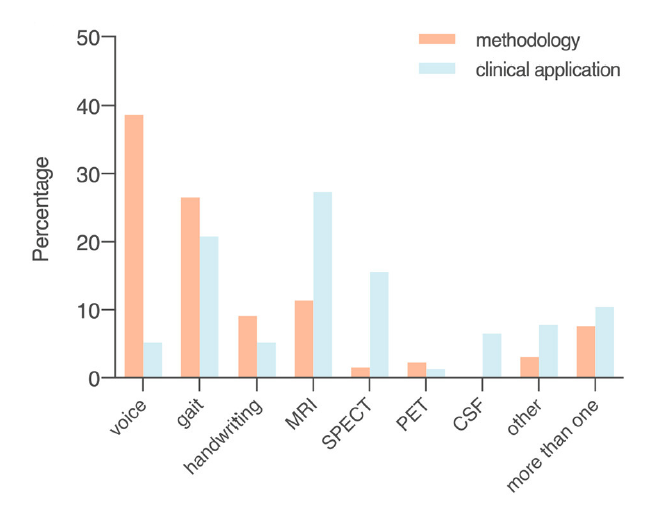
\includegraphics[width=0.6\textwidth]{./img/plot_PD_detection_methods}~\caption{Wykorzystanie rozwiązań w opracowaniach teoretycznych i zastosowaniach klinicznych w zależności od rodzaju danych (stan na dzień 14 luty 2020) \cite{ML_for_PD_review} }
    \label{fig:pd_detection_methods}
\end{figure}


Rysunek \ref{fig:pd_detection_methods} ilustruje zastosowanie wymienionych metod zarówno w teorii, jak i praktyce.
Metody oparte na obrazowaniu medycznym wykazują wyraźną przewagę w zastosowaniach klinicznych w porównaniu do kontekstu teoretycznego.
Niemniej jednak, to pozostałe metody budzą znacznie większe zainteresowanie ze strony środowiska naukowego.
Szczególnie w przypadku analizy głosu, gdzie rozbieżność między teorią a praktyką jest szczególnie znacząca.
Przyczyny tego zjawiska zostaną dokładniej rozważone w dalszej części pracy.
Co ciekawe, jak przedstawiono na wykresie \ref{fig:pd_accuracy_methods}, detekcja choroby na podstawie głosu daje bardzo wysokie wyniki,
w większości analizowanych artykułów.

\begin{figure}[htbp]
	\centering
	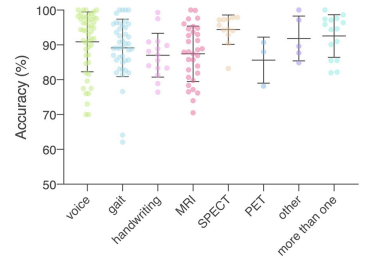
\includegraphics[width=0.6\textwidth]{./img/accuracy}~\caption{Dokładność rozwiązań diagnostycznych w zależności od rodzaju danych (stan na dzień 14 luty 2020) \cite{ML_for_PD_review} }
    \label{fig:pd_accuracy_methods}
\end{figure}

Opracowanie dotyczy diagnostyki opartej na analizie głosu, dlatego temat ten zostanie bliżej rozważony.
Założeniem dla takich systemów jest zadanie potencjalnemu pacjentowi zadania wokalnego, może to być:
\begin{itemize}[itemsep=0.1pt]
	\item podtrzymywane samogłoski (ang. \emph{sustained vowels}),
	\item zadanie diadochokinetyczne (DDK), mogące mierzyć zdolność do wydawania serii szybkich i naprzemiennych dźwięków (sylab),
	\item czytanie tekstu,
	\item wypowiedzenie pojedynczego zdania,
	\item monolog.
\end{itemize}

Dotychczas nie przeprowadzono badań porównawczych dotyczących wpływu wyboru zadania wokalnego na efektywność klasyfikacji w przypadku choroby Parkinsona (PD).
Jedynie w artykule  \cite{vocal_task_comparision} przeprowadzono takie porównanie, przy użyciu cech prozodii.
Nie pozwala to jednak na wyciągnięcie obiektywnych wniosków, ponieważ każde z zadań wokalnych może wymagać innego podejścia i metod klasyfikacji.
Niemniej jednak, autorzy publikacji \cite{monitoring_speech} przeprowadzili badanie na 200 pacjentach z PD,
gdzie dokonano klasyfikacji deficytów mowy na pięć poziomów nasilenia.
Oceniono typ (głos, artykulacja, płynność) oraz zakres upośledzenia dla każdego poziomu, korzystając z 2-minutowego fragmentu mowy.
Wyniki ukazały, że głos stanowił najczęściej występujący i bardziej nasilony deficyt we wczesnych stadiach choroby.
Deficyty artykulacji i płynności pojawiały się później.
Wykazano, że upośledzenie artykulacji korelowało z upośledzeniem głosu w fazie "ciężkiej", a w fazie "głębokiej" dominującą cechą była upośledzona artykulacja.

W rezultacie, w kontekście wczesnej diagnostyki choroby, artykulacja i płynność mowy nie wymagają głębokiej uwagi.
Koncentrację należy skupić przede wszystkim na cechach głosowych, co sprawia, że wybór podtrzymywanych samogłosek jako zadania wokalnego
wydaje się być najlepszym wyborem ze względu na ich stabilność w czasie oraz łatwość wypowiadania przez pacjenta.
To podejście może posiadać potencjał uniwersalności dla różnych języków, co oznacza, że analiza może być stosowana
niezależnie od języka ojczystego pacjenta.
W efekcie pozwala to na bardziej efektywne i znormalizowane diagnozowanie choroby Parkinsona.

Najczęściej występującymi w opracowaniach samogłoskami są /a/, /e/, /i/ oraz /u/.
Aktualnie brakuje albo nie udało się jeszcze ustalić, która z tych samogłosek niesie najcenniejsze informacje z punktu widzenia diagnostycznego.
W związku z tym, w ramach badawczej części niniejszej pracy przeprowadzone zostanie takie porównanie dla wybranych metod.
%---------------------------------------------------------------------------

\section{Metody klasyfikacji}\label{sec:metody-klasyfikacji}

W publikacji \cite{ML_for_PD_review} dokonano przeglądu wykorzystania metod uczenia maszynowego w automatycznej diagnostyce choroby Parkinsona.
Spośród 55 wybranych artykułów opublikowanych do lutego 2020 roku 49 badań osiągnęło średnią dokładność na poziomie 90,9\%,
wahając się od 70,0\% \cite{7378178, multimodel-framework} do 100,0\% \cite{new-hybrid, fuzzy-neural-system, linear-discriminant-analysis, dastjerd}.
Eksperymenty były przeprowadzane na różnych bazach danych, co czyni je trudne do wzajemnego porównania.
Wykorzystywały różne zadania wokalne, a tym samym różne podejścia do problemu.

W zależności od przyjętego podłoża diagnostycznego dobiera się odpowiednią metodę klasyfikacji.
Różne metody okażą się skuteczne w przypadku analizy mowy spontanicznej w porównaniu do mowy kontrolowanej.
Dlatego w tej części pracy zostaną przedstawione metody klasyfikacji związane z podtrzymywaniem samogłosek, które to zostały wybrane jako
fundament badawczy w ramach niniejszego opracowania.

Najpowszechniejszym podejściem do automatycznej diagnostyki choroby Parkinsona na podstawie głosu jest tzw. tradycyjna inżynieria cech.
To proces wydobywania z sygnału mowy charakterystycznych cech, takich jak formanty, jitter, współczynniki cepstralne MFCC, stosunek harmoniczny do
szumów (NHR), stosunek harmoniczny do szumów (HNR), wskaźnik migotania Shimmer, częstotliwość podstawowa i inne.
Chociaż to podejście jest powszechne, to istnieją także inne, bardziej zaawansowane metody.

Jedną z nich jest wykorzystanie spektrogramów jako podstawy dla procesu klasyfikacji.
Ten proces polega na przekształceniu dźwięków mowy na formę wizualną w postaci spektrogramów, które prezentują zmiany w czasie i częstotliwości.
Następnie, w celu klasyfikacji, można wykorzystać sieci konwolucyjne, które są specjalnie zaprojektowane do pracy z obrazami.
Analizują one strukturę i wzorce w spektrogramach, umożliwiając rozróżnienie cech charakterystycznych dla różnych stanów zdrowotnych.
To podejście może przyczynić się do szybszej i bardziej precyzyjnej diagnostyki poprzez analizę cech mowy, które mogą być trudne do wykrycia za pomocą
innych metod.

W publikacji \cite{Majda-Zdancewicz_Potulska-Chromik_Jakubowski_Nojszewska_Kostera-Pruszczyk} dokonano porównania tradycyjnego podejścia opartego na
inżynierii cech z nowoczesnym wykorzystaniem zaawansowanych głębokich sieci neuronowych.
Wyniki wskazały, że głęboka sieć konwolucyjna AlexNet osiągnęła wrażliwość na poziomie 93,2\% i swoistość na poziomie 79,5\%, podczas gdy inżynieria
cech dawała wrażliwość na poziomie 97,7\% i swoistość na poziomie 93,2\%.
Autorzy sugerują, że połączenie tych podejść może zwiększyć skuteczność.
Mimo że podejście oparte na tradycyjnej inżynierii cech dało lepsze wyniki, istnieje potencjał uzyskania lepszych rezultatów poprzez wykorzystanie
głębszych sieci, takich jak te z rodzin VGG i ResNet.

Większość publikacji w analizowanym obszarze dotyczy niewielkich zbiorów danych (mniej niż 50 nagrań).
Wynika to z małej dostępności otwartych baz danych i może wiązać się z nieobiektywnymi wynikami.
W badaniu \cite{GUATELLI2023106700}, bazującym na bazie danych 135 osób, wyniki mieściły się między 81,74\% a 83,91\% dokładności,
przy wykorzystaniu konwolucyjnych sieci neuronowych (ang. \emph{Convolutional Neural Networks}, CNN) oraz ELM (ang. \emph{Extreme Learning Machines}).
Analiza pokazała, że większa liczba próbek wpływa na lepsze wyniki, a sieć AlexNet miała najlepszą równowagę między rozproszeniem a wydajnością.

W innym badaniu \cite{Gelvez-Almeida_2022} przeanalizowano różne wersje ELM w celu klasyfikacji pacjentów z chorobą Parkinsona na podstawie 135 spektrogramów.
Wyniki wskazują, że wielowarstwowe sieci ELM wykazują lepszą wydajność niż jednowarstwowe.
Osiągnięto dokładność, oscylującą w okolicach 80\%.

Ciekawą analizę opisano w publikacji \cite{8999815}. Zaproponowano trzy podejścia - pierwsze oparte o transfer learning, wykorzystujące spektrogramy nagrań
mowy; drugie, wykorzystujące głębokie cechy wyodrębnione ze spektrogramów mowy za pomocą klasyfikatorów uczenia maszynowego; oraz trzecie, oceniające
proste cechy akustyczne nagrań również przy użyciu klasyfikatorów uczenia maszynowego.
Wyniki wskazują, że druga propozycja wykazuje obiecujące rezultaty.
Zaobserwowano najwyższą dokładność na poziomie 99,7\% dla samogłoski \textbackslash o\textbackslash\ oraz odczytywanego tekstu przy użyciu perceptronu wielowarstwowego.
Natomiast dla głębokich cech samogłoski \textbackslash i\textbackslash\ uzyskano dokładność wynoszącą 99,1\% przy użyciu lasu losowego.
Metoda bazująca na głębokich cechach wykazuje lepsze wyniki w porównaniu do prostych cech akustycznych i podejść opartych na transfer learning.
Zaproponowana metodologia przewyższa istniejące techniki na zbiorze danych PC-GITA w wykrywaniu choroby Parkinsona.

W publikacji \cite{9257451}  zaproponowano  wykorzystanie \emph{Spectrogram-Deep Convolutional Generative Adversarial Network} (S-DCGAN)
do augmentacji próbek w celu przezwyciężenia ograniczonej ilości istniejących zestawów danych pacjentów oraz próbek głosowych.
S-DCGAN generuje spektrogram wysokiej rozdzielczości poprzez zwiększenie warstw sieci, dodanie metody normalizacji spektralnej (ang. \emph{Spectral Normalization}, SN) oraz
zastosowanie strategii dopasowania cech.
Wybierane są spektrogramy o wysokim podobieństwie i niskim zniekształceniu na podstawie wartości wskaźnika strukturalnej
indywidualności (ang. \emph{Structural Similarity Index}, SSIM) oraz stosunku sygnału do szumu maksymalnego (ang. \emph{Peak Signal to Noise Ratio}, PSNR)
w celu augmentacji próbek.
Wykorzystano model ResNet50 z warstwą globalnego uśredniania (ang. \emph{Global Average Pooling}, GAP) do ekstrakcji cech głosowych i skutecznej
klasyfikacji.
GAP eliminuje problem nadmiernego dopasowania i przyspiesza optymalizację.
Ostatecznie, na zestawie danych Sakar, hybrydowy model S-DCGAN-ResNet50 osiągnął najwyższą dokładność rozpoznawania wzorca głosowego wynoszącą 91,25\%
oraz swoistość na poziomie 92,5\%, co pozwala na precyzyjniejszą różnicowanie między pacjentami z PD a zdrowymi osobami w porównaniu z modelem
DCGAN-ResNet50.
Rozszerza to środowisko stosowania rozpoznawania wzorca głosowego w dziedzinie medycyny i umożliwia jego uniwersalność w różnych
zestawach danych.

W badaniu \cite{ER2021103006} zaproponowano nowe podejście oparte na wcześniej wytrenowanych głębokich sieciach i długoterminowej pamięci krótkoterminowej (LSTM),
wykorzystujące mel-spektrogramy.
Zaproponowany model składa się z czterech etapów.
W pierwszym kroku usuwany jest szum  poprzez zastosowanie rozkładu modalnego wariacyjnego (VMD).
W drugim etapie z sygnałów dźwiękowych ulepszonych za pomocą VMD wyodrębniane są mel-spektrogramy.
W trzecim etapie wykorzystywane są wcześniej wytrenowane głębokie sieci do ekstrakcji głębokich cech z mel-spektrogramów.
W tym celu używane są modele ResNet-18, ResNet-50 i ResNet-101.
W ostatnim etapie proces klasyfikacji zachodzi poprzez podanie tych cech jako wejścia do modelu LSTM, który jest zaprojektowany do wyodrębniania
informacji sekwencyjnych z wyekstrahowanych cech.
Eksperymenty przeprowadzono na zestawie danych PC-GITA.
Dokładność uzyskana za pomocą zaproponowanej metody wynosi 98.61\%.



%---------------------------------------------------------------------------

\section{Wyzwania związane z systemami automatycznej diagnostyki}\label{sec:wyzwania}

Zainteresowanie systemami do automatycznej diagnostyki choroby Parkinsona na podstawie głosu jest ogromne i wiąże się z nim duże nadzieje.
Istnieje jednak duża dysproporcja pomiędzy pracą badawczą a ich wykorzystaniem w rzeczywistym środowisku Rys \ref{fig:pd_detection_methods}.
Przyczyn takiego stanu rzeczy jest wiele, a większość z nich związana jest z brakiem usystematyzowanego podejścia do problemu, co utrudnia porównanie
rozwiązań, a tym samym rzetelny postęp.

Ostatnie badania wykazały, że możemy wytrenować dokładne modele do wykrywania oznak PD z nagrań audio.
Jednakże, istnieją rozbieżności, które są częściowo powodowane przez różnice w
wykorzystywanych korpusach lub metodologii.
Dlatego autorzy publikacji \cite{SustainedVowelsProblems} przeprowadzili analizę, wpływu niektórych czynników na wyniki klasyfikacji.
Głównym celem artykułu była ich identyfikacja oraz stworzenie zasad, które w przyszłości pozwolą usystematyzować
stan wiedzy w tej dziedzinie.
W badaniach skupiono się na przedłużonych samogłoskach (ang. \emph{sustained vowels}), ponieważ są one najlepszym i najpopularniejszym zadaniem
wokalnym w takich systemach.
Przeprowadzone eksperymenty wykazały, że nieuwzględnione zmienne w metodologii, projekcie eksperymentalnym i
przygotowaniu danych prowadzą do zbyt optymistycznych wyników w badaniach nad automatyczną detekcją PD.
Czynniki, które zidentyfikowano jako przyczyniające się do zbyt optymistycznych wyników klasyfikacji
przedstawiono na Rys. \ref{fig:factors_PD_detection} oraz omówiono poniżej.


\begin{figure}[htbp]
	\centering
	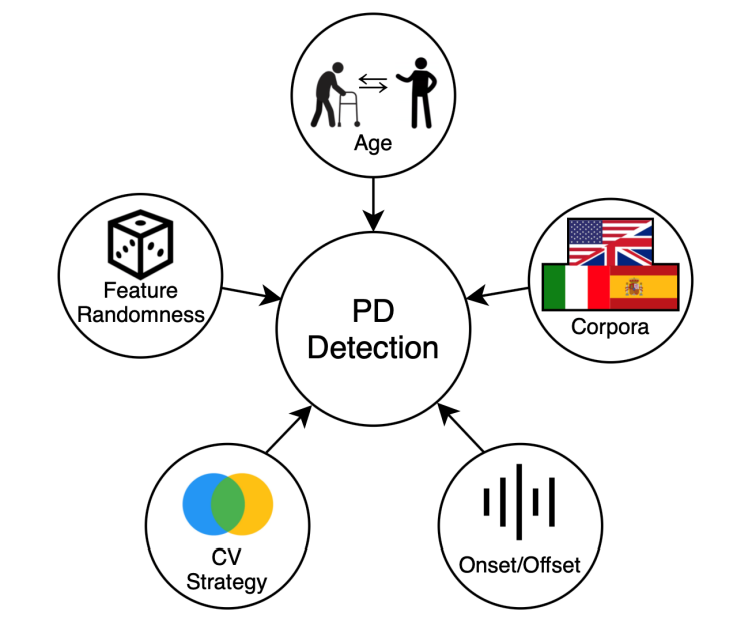
\includegraphics[width=0.4\textwidth]{./img/influence_of_factors_on_PD_detection}
	\caption{Czynniki wpływające na dokładność detekcji PD na podstawie głosu \cite{SustainedVowelsProblems}}
    \label{fig:factors_PD_detection}
\end{figure}


\begin{enumerate}[label={\alph*)}]
	\item Pominięcie aspektu tożsamości mówcy przy konstruowaniu zbiorów treningowych i testowych
	\item[] W przypadku, gdy w zbiorze danych znajduje się kilka nagrań od tego samego mówcy można postąpić na dwa sposoby.
Pierwszy z nich to podział według podmiotów (ang. \emph{subject-wise split}) polegający na tym, że nagrania od tej samej
osoby znajdują się albo w zbiorze treningowym albo testowym - nigdy w obu na raz.
Drugie podejście to podział według rekordów (ang. \emph{record-wise split}), gdzie nagrania są losowo dzielone do zbiorów
lub intencjonalnie używa się nagrań od tej samej osoby zarówno w zbiorze testowym jak i treningowym.
Okazuje się, że podejście typu \emph{record-wise} prowadzi do wyższej dokładności niż \emph{subject-wise split}, jeśli pozostałe założenia pozostają identyczne.
Prawdopodobnie wynika to z faktu, że klasyfikator nastawia się na wykrywanie unikalnych informacji indywidualnych,
reprezentowanych przez współczynniki takie jak MFCC, a nie rzeczywiste biomarkery lub wzorce PD.
Dlatego też rekomendowana jest technika \emph{subject-wise split}, aby uniknąć zbyt optymistycznych wyników.

  	\item Niezbalansowanie klas pod względem wieku
	\item[] W literaturze można znaleźć prace wykorzystujące zbiory danych, w których średni wiek mówców
w klasie osób chorych na PD różni się od średniego wieku w klasie osób zdrowych o ponad 5 lat.
Autorzy zapewniają o wysokiej skuteczności swoich rozwiązań, jednak pomijają informacje o ryzyku, że klasyfikator
uczy się wykrywać cechy powiązane z wiekiem, zamiast rzeczywistych wzorców PD.
Wyniki eksperymentów w publikacji \cite{SustainedVowelsProblems} pokazują, że wraz ze wzrostem różnicy między średnim wiekiem uczestników z PD i HC,
dokładność klasyfikacji konsekwentnie rośnie (Rys. \ref{fig:acc_and_age_diff}).
Na tej podstawie można stwierdzić, że związany z wiekiem wpływ na głos mówców może zaburzać wyniki otrzymywane przez klasyfikator.
Dlatego też zaleca się zbalansowanie używanych zbiorów danych, tak aby średnia różnica wieku między tymi dwoma klasami była jak namniejsza.


\begin{figure}[htbp]
	\centering
	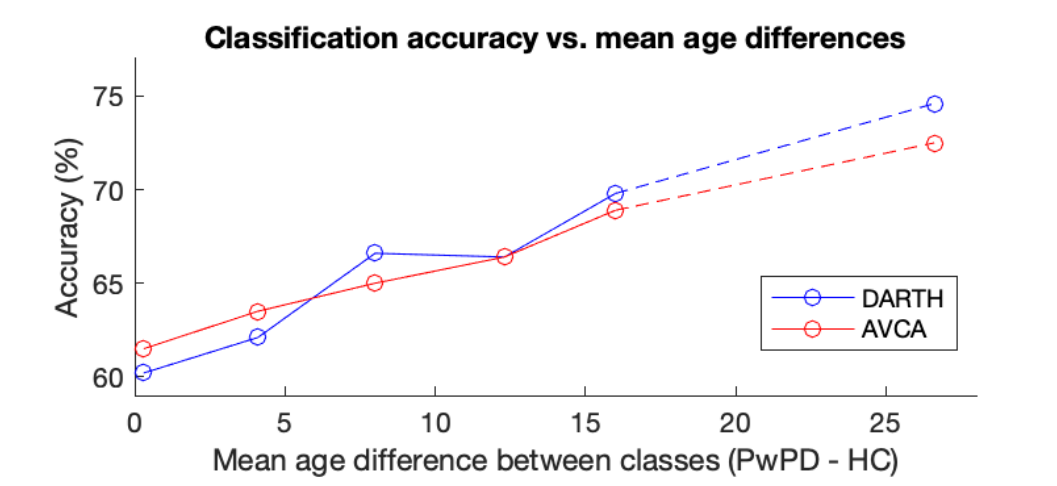
\includegraphics[width=0.7\textwidth]{./img/acc_and_age_difference}
	\caption{Wykres przedstawiający zależność różnicy wieku między klasami a dokładnością klasyfikacji \cite{SustainedVowelsProblems}}
    \label{fig:acc_and_age_diff}
\end{figure}

  	\item wpływ losowości cech na dokładność klasyfikacji
	\item[] W publikacji \cite{SustainedVowelsProblems} przeprowadzono badania analizujące wpływ losowości cech na dokładność klasyfikacji.
Zamieniono cechy obliczone za pomocą DARTH-VAT na losowe liczby, zachowując etykiety i podziały.
Wyniki wskazały, że nawet losowe cechy mogą prowadzić do wysokich wyników klasyfikacji (ponad 72\%).
Efekt ten jest bardziej widoczny w mniejszych korpusach, gdzie różnica między liczbą nagrań a wymiarowością cech ma większy wpływ na potencjalną korelację przypadkową.
Badanie pokazuje, że nadmierna liczba cech w stosunku do liczby obserwacji może prowadzić do fałszywie wysokich wyników klasyfikacji nawet przy użyciu losowych cech.
Im większa różnica między liczbą plików a wymiarem wektora cech, tym większe szanse na znalezienie cechy, która losowo koreluje z etykietami klas.
To sugeruje, że osiągnięcia klasyfikacyjne powinny być analizowane w kontekście proporcji cech do próbki, aby uniknąć nadmiernie optymistycznych interpretacji wyników klasyfikacji w zastosowaniach medycznych.

  	\item ograniczenie losowego nadmiernego dopasowania poprzez uwzględnienie zbioru walidacyjnego
	\item[] Dla mniejszych zbiorów danych, praktyką jest często używanie tylko zbiorów treningowych i testowych podczas krzyżowej walidacji.
Jest to podejście, które może prowadzić do wyników zbyt optymistycznych, ponieważ wszystkie wyniki testowe są brane pod uwagę przy wyborze optymalnej
konfiguracji modelu.
Inną strategią jest wykorzystanie danych treningowych do oceny wytrenowanych modeli i późniejsze przetestowanie najlepszego modelu na zbiorze testowym.
Niemniej jednak, to podejście może być niepraktyczne, ponieważ może prowadzić do wyników idealnych (dokładność 100\%) na zbiorze treningowym, co jest niepożądane.
Aby uniknąć tych problemów, proponuje się wykorzystanie dodatkowego zbioru walidacyjnego \cite{SustainedVowelsProblems}.
Wybierając model na podstawie wyników walidacyjnych, a następnie testując go na zbiorze testowym, można uniknąć ryzyka nadmiernego dopasowania.
Dla mniejszych zbiorów danych, ta strategia może ograniczać dostępną liczbę danych treningowych, co wpływa na wydajność klasyfikacji.

	\item wpływ początku i końca  nagrań samogłosek na wyniki klasyfikacji
\item[] Główną różnicą między korpusami wykorzystywanymi do klasyfikacji choroby Parkinsona (PD) jest obecność fragmentów nagrania oznaczonych jako "onset" i "offset".
Niektóre nagrania zawierają te segmenty, podczas gdy inne zostały ich pozbawione, aby zapewnić stabilniejszą fonację, co jest korzystne dla pewnych cech i algorytmów analizy.
W celu oceny znaczenia informacji zawartych w obszarach "onset" i "offset" dla klasyfikacji, przeprowadzono eksperymenty porównawcze,
wykorzystując nagrania zarówno z fragmentami przyciętymi, jak i nieprzyciętymi \cite{SustainedVowelsProblems}.
Wyniki tych eksperymentów ukazały, że wyeliminowanie fragmentów początkowych i końcowych wpłynęło negatywnie na dokładność klasyfikacji.
To wskazuje na to, że obszary te zawierają istotne informacje artykulacyjne, które mają znaczenie dla procesu klasyfikacji.

 	\item eksperymenty międzykorporowe a zdolności generalizacyjne
	\item [] Większość badań dotyczących diagnozowania choroby Parkinsona na podstawie głosu opiera się na jednym, lub ewentualnie kilku (wykorzystywanych niezależnie)
korpusach mowy.
W tym kontekście często pomija się badanie zdolności klasyfikatorów do ogólnego zastosowania.
W artykule \cite{SustainedVowelsProblems} przeprowadzono międzykorporowe eksperymenty na bazach danych w językach włoskim i hiszpańskim w celu
przetestowania zdolności ogólnych modeli. Skuteczność tych modeli różniła się w zależności od języka zbioru testowego.
Może to wynikać z odmiennej różnorodności nagrań, co ma wpływ na stabilność modelu.
Drugim możliwym wyjaśnieniem jest to, że głos osób z chorobą Parkinsona może być w różnym stopniu obarczony objawami choroby w zależności od języka ojczystego lub stopnia zaawansowania choroby.
Innymi słowy, w zależności od użytego zbioru danych objawy mogą być nasilone w różny sposób i konieczne jest wzięcie tego pod uwagę tak by zdolności generalizacyjne modelu były jak najwyższe.
\end{enumerate}


Identyfikacja i świadomość wpływu powyższych czynników, pozwala na dostosowaniu przeprowadzanych ekperymentów tak, aby uniknąć wyników zbyt optymistycznych.
Usystematyzowanie podejścia do analizy głosu pod kątem diagnostyki choroby Parkinsona przyczyni się do możwliwości obiektywnego porównania istniejących i nowych rozwiązań.
Tym samym przyspiesy to postęp w tej dziedzinie i uzyskanie optymalnego rozwiązania, które mogłoby zostac wykorzystane w rzeczywistym środowisku.

Nie są to jednak wszystkie czynniki, które zaburzają obiektywność wyników. Konieczna jest dyskusja na temat nowych
kompleksowych linii bazowych dla prowadzenia eksperymentów w automatycznym wykrywaniu PD na podstawie fonacji,
a także innych ogólnych zastosowań przetwarzania mowy.

Prace nad automatyczną detekcją Parkinsona na podstawie głosu trwają już od dłuższego czasu.
Jednak wciąż brakuje systemu, który mógłby zostać uznany jako wystarczajaco niezawodne narzędzie diagnostyczne.
Wśród problemów, które ograniczają rzeczywiste wykorzystanie takich systemów wyróżnia się:
\begin{itemize}[itemsep=0.1pt]
	\item zróżnicowanie wzorców mowy: osoby z chorobą Parkinsona mogą różnić się w sposób, w jaki zmiany w mowie wpływają na ich głos.
To zróżnicowanie utrudnia stworzenie uniwersalnego modelu, który działałby skutecznie dla wszystkich pacjentów.
	\item wpływ zmiennych czynników: wpływ na mowę mogą mieć różne czynniki, takie jak zmęczenie, stres czy otoczenie akustyczne.
Te zmienne mogą wprowadzać zakłócenia w analizie mowy i utrudniać jednoznaczną diagnozę.
	\item potrzeba dużej bazy danych: aby stworzyć dokładny system detekcji, konieczne jest posiadanie dużej bazy danych głosów osób z i
bez choroby Parkinsona. Uzyskanie takiej bazy danych, która odzwierciedla różnorodność pacjentów i warunki środowiskowe, może być wyzwaniem.
Większość publikacji opiera się na bazach danych zawierających około 50 nagrań, co nie jest wystraczająco reprezentatywną próbą.
	\item wczesne wykrycie i subtelne objawy: wczesne stadia choroby Parkinsona często manifestują się subtelnie, a różnice w mowie mogą być
trudne do zauważenia. To może prowadzić do błędnych diagnoz lub niskiej skuteczności systemu.
	\item weryfikacja i walidacja: Aby narzędzie diagnostyczne oparte na mowie było skuteczne, musi być poddane rygorystycznym testom w rzeczywistych
warunkach klinicznych. Weryfikacja i walidacja takiego systemu to skomplikowany proces.
	\item ograniczenia technologiczne: pomimo postępów w technologii analizy mowy, istnieją nadal ograniczenia w dokładności i precyzji takich systemów.
Może to prowadzić do wyników fałszywie pozytywnych lub negatywnych.
	\item aspekty etyczne i prywatność: wykorzystywanie danych głosowych do diagnozowania chorób podnosi kwestie związane z prywatnością i etyką.
Konieczne jest zagwarantowanie odpowiednich zabezpieczeń danych i zgody pacjentów na wykorzystanie ich informacji w celach medycznych.
\end{itemize}

Mimo tych wyzwań, prace nad wykorzystaniem analizy mowy do diagnozowania choroby Parkinsona są obiecujące i mogą przyczynić się do poprawy jakości życia
pacjentów oraz usprawnienia procesu diagnozy i leczenia.
Jednakże przed stworzeniem skutecznego narzędzia diagnostycznego opartego na głosie jest jeszcze wiele pracy do wykonania

W niniejszej pracy podjęta zostanie próba implementacji takiego rozwiązania.
Uwzględnione zostaną wszystkie z rekomendacji przedstawionych w artykule \cite{SustainedVowelsProblems}.
%---------------------------------------------------------------------------
